\section{Локалізація рухомих об'єктів}

Розглянемо теоретичне підґрунтя методів, які використовуються в даній роботі для
локалізації рухомих об'єктів, а саме задачу Min-Cut/Max-Flow, та її рішення
у вигляді алгоритму Бойкова-Колмогорова.

\subsection{Задача знаходження Min-Cut/Max-Flow}

Перед описом алгоритму Бойкова-Колмогорова варто зрозуміти яку конкретну
задачу він вирішує. Існує проблема знаходження мінімального зрізу або їй
еквівалентна максимального потоку. Дана задача базується на концепції
трубопроводів. Є мережа труб, кожна з яких має свою пропускну здатність
та потік води, що вона пропускає. У даній мережі є джерело води та стік(кінець мережі).
Головна задача - знайти максимальний потік, який потрібно пропустити через джерело,
щоб ефективно використовувати трубопроводи.

Якщо дану концепцію перекласти у мову
математики, то мережею трубопроводів є граф $G$ (Рис. \ref{fig:graph_example})
з множинами вузлів $T$ та направлених дуг(ребер) $\tau$. В ньому є джерело $s$,
стік $e$, дві множини дуг $N_t = \{t^{'}: tt^{'} \in \tau \}$ та $P_t = \{t^{'}: t^{'}t \in \tau \}$,
які складають $\tau$. Потік позначатимемо як $f$, а пропускну здатність $c$.

\begin{figure}[H]
    \centering
    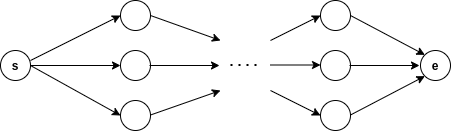
\includegraphics[width=0.5\textwidth]{images/graph_example}
    \caption{Приклад графу
        \label{fig:graph_example}
    }
\end{figure}

Задача максимального потоку формулюється так:

\begin{equation*}
    \sum_{t \in N_s} f_{st} \rightarrow \max_{f: \tau \rightarrow R }
\end{equation*}

З обмеженнями:
\begin{equation*}
    \begin{gathered}
        \begin{cases}
            f_{tt^{'}} \leq  c_{tt^{'}},                                   & \forall tt^{'}  \in \tau ,         \\
            \sum_{p \in P_t} f_{pt} - \sum_{t^{'} \in N_t} f_{tt^{'}} = 0, & \forall t \in T \setminus \{s,e\}, \\
            \sum f_{tt^{'}} \geq 0,                                        & \forall tt^{'}  \in \tau
        \end{cases}
    \end{gathered}
\end{equation*}

Що значить:
\begin{enumerate}
    \item Потік має не перевищувати пропускну здатність для всіх ребер;
    \item Сума потоків, що входять у вузол не повинна змінитись на виході;
    \item Потік завжди додатній.
\end{enumerate}

Як вже було зазначено розв'язавши задачу, максимального потоку одночасно вирішується і задача
мінімального зрізу. Даний висновок отримується з Max-Flow Min-Cut теореми.
Мінімальним зрізом є множина тих ребер, які стали насиченими після знаходження максимального
потоку. Тобто мінімальний зріз створює дві множини, що формують множину всіх дуг.

Вирішення Min-cut/Max-Flow задачі може базуватись на двох принципах:
з використанням пошуку в глибину (Едмондса-Карпа) або пошуку в ширину (Форда-Фалкерсона).
\begin{algorithm}[H]
    \caption{Алгоритм Min-Cut/Max-Flow}
    \begin{algorithmic}
        \State \textbf{Вхід:} Граф, з об'єктами $ t \in T $, ребрами $tt^{'} $
        \State \textbf{Вихід:} $ F_{maxflow} $ - значення максимального потоку;
        \State \textbf{Ініціалізація:} $ F_{maxflow} = 0, f_{tt^{'}}^{0} = 0 \quad \forall tt^{'}  \in \tau $.
        \State \textbf{Поки існує шлях з $s$ в $e$ повторюємо кроки 1,2:}
        \State \textbf{Крок 1:} Знаходимо шлях від $s$ до $e$ (пошуком в ширину чи в глибину).
        \State Відвідуємо $ t^{'}$ із $t $ якщо:
        \State \qquad 1. $ f_{tt^{'}} \neq c_{tt^{'}} $
        \State \qquad 2. $ \nexists p_{t^{'}}^{i} \Rightarrow p_{t^{'}}^{i} = t $ (запам'ятали вершину)
        \State \qquad 3. $ t^{'} \neq s $
        \State \textbf{Крок 2:} Проходимо по заданому шляху:
        \State \qquad 1. Знаходимо $ \vartriangle f^{i} = \min_{tt^{'} \in \{шлях із s в e \}} $
        \State \qquad 2. Змінюємо потік: $ f_{tt^{'}}^{i+1} = f_{tt^{'}}^{i} + \vartriangle f^{i} $
        \State \qquad 3. Оновлюємо $ F_{maxflow}: F_{maxflow}^{i+1} = F_{maxflow}^{i} + \vartriangle f^{i} $
    \end{algorithmic}

    Знайшовши максимальний потік, можемо знайти і мінімальний зріз: \\
    Для $\forall t \in T$ знайти $\theta_{t} \in \{0,1\}$
    \begin{algorithmic}
        \State \textbf{Крок 3}: Запускаємо пошук в ширину або глибину вже з оновленим графом.
        \State \qquad Якщо $c_{tt^{'}} \geqslant f_{tt^{'}}$ та $c_{tt^{'}} \geqslant 0$
        $\Rightarrow \theta_{t^{'}} = 1 $, інакше $\theta_{t^{'}} = 0 $
    \end{algorithmic}
\end{algorithm}

У 2004 році Юрій Бойков та Володимир Колмогоров запропонували свій підхід \cite{boykov_kolmogorov}
у вирішенні Max-Flow/Min-Cut задачі.
Запропонована ідея методу полягає в огментації шляхів. Будується два дерева $S$ та $T$
коренями яких є $s$ та $t$ відповідно. Вершини загально діляться на ті що в $S$, $T$, та
\textit{вільні}. Кожне дерево має \textit{активні} та \textit{внутрішні} вершини.
\textbf{Алгоритм Бойкова-Колмогорова} складається зі стадій \textit{росту},
\textit{огментації}, \textit{всиновлення}.\\
Коротко розглянемо кожну з них:

\begin{enumerate}
    \item \textbf{Стадія Росту} \\
          Проводимо одночасний ріст дерев з вершин $s$ та $e$, знаходимо активні
          вершини і додаємо їх як вершини, що відвідали. Після такого сканування вершини
          стають внутрішніми. Цей процес продовжується поки не залишиться не активної вершини.
    \item \textbf{Стадія Огментації} \\
          На цій стадії шлях, що був знайдений на попередньому етапі огментується(розділення)
          по ребру залишкової пропускної здатності (\textit{bottleneck}). Якщо ребра дерева стають
          насиченими (пропускна здатність = потоку) найвіддаленіші вершини від коренів дерев стають
          \textit{сиротами}. Тобто, якщо наприклад вершини $t$ та $t^{'}$ знаходяться в дереві $S$
          і ребро $(t,t^{'})$ є насиченим, тоді $t^{'}$ називається \textit{$S$ - сиротою}.
          Аналогічно, якщо $t$ та $t^{'}$ знаходяться в дереві $T$, то  $t$ - \textit{$T$ - сирота}.
          Якщо ребро знаходиться в \textit{bottleneck}( $t$ в $S$, $t^{'}$ в $T$, ребро $(t,t^{'})$
          насичене) відповідно немає ніяких сиріт. Всі сироти потрапляють у список сирот.
    \item \textbf{Стадія Всиновлення} \\
          На даному етапі ми проходимось по кожній сироті в списку сирот для кожного дерева.
          Нехай $t^{'}$ \textit{$S$ - сирота}. Знаходимо всі $t$  в $S$, які формують ребро
          ($t$, $t^{'}$). Для кожного такого $t$ перевіряємо чи шлях з $t$ в $s$ містить сироти
          включаючи $t$. Якщо сирот не знайшли, то $t$ - батько  $t^{'}$. \\
          Якщо не вдається знайти батька, ми позначаємо вершину $t^{'}$ як \textit{вільну}, а всіх
          дітей $t^{'}$ сиротами. Після цього ми оброблюємо залишкові ребра $(t,t^{'})$ і для кожного $t$ в $S$ позначаємо
          $t$ - активною.
\end{enumerate}


\begin{figure}[h]
    \centering
    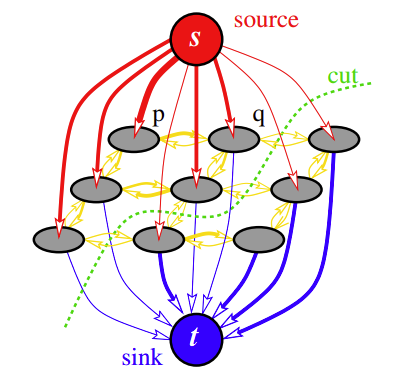
\includegraphics[width=0.3\textwidth]{images/graph_cut}
    \caption{Приклад графу-решітки з мінімальним розрізом
        \label{fig:graph_lattice}
    }
\end{figure}

Найбільша перевага даного алгоритму це те що, він працює швидше та краще на графах-решітках
(Рис. \ref{fig:graph_lattice}).
Оскільки саме таку структуру ми використовуємо в алгоритмі Б-К для отримання маски рухомих
об'єктів це дає змогу оброблювати кадри відео досить швидко.
